\label{Chapter:Evaluation of the User Study}
In the previous chapter we saw the study design and procedure. Based on this we planned to conduct the user study with 10 participants. However, 1 participant had to drop out which left us with 9 participants. The demographics showed us that they were between the ages of 22 and 33 with 7 out of 9 of them under the age of 30. 3 out of 9 participants were female. In this chapter we will evaluate and discuss the findings of the study and then look at what insights this gives about the possible uses of our automated guided jumping technique. While explaining the results we will refer to the two techniques for the study tasks as \textbf{FJ} for the \textbf{Free Jumping} condition and \textbf{AJ} for the \textbf{Automated Jumping} condition. We will also represent mean averages, median values and standard deviations with their common symbols which are \textbf{Avg}, \textbf{Mdn} and \textbf{$\sigma$} respectively. These values will all be rounded to the nearest hundredths. Individual participants will be referred to as \textbf{P}$_n$ where n is the participant number.

\section{User Comfort}
\label{subsection EUS: User Comfort}
During the study none of the participants felt too sick that they could not continue with it. The maximum discomfort score was 4 during AJ when the participant had this condition in their second task. Overall, there was a positive skew for discomfort score during both conditions as can be seen in \cref{fig:user-comfort}(1). However, the FJ condition was more positively skewed and had lower simulator sickness than AJ ($Avg_{FJ}$ = 0.67, $Mdn_{FJ}$ = 0, $\sigma_{FJ}$ = 0.86; $Avg_{AJ}$ = 1.33, $Mdn_{AJ}$ = 1, $\sigma_{AJ}$ = 1.5). It also seems as if the he order in which the conditions were presented to participants did not impact the discomfort score as for most participants AJ always has a higher discomfort score regardless of when it was presented. While this proves \cref{hyp:hyp1} false, we do see that the simulator sickness for AJ is not that bad, even if it was worse than for FJ, and hence our technique still manages to avoid excessive simulator sickness.

In addition to the discomfort score we also got results for the general user comfort which showed that it was better for FJ as can be seen in \cref{fig:user-comfort}(2). Both the conditions show a negative skew with the results for FJ more negatively skewed than for AJ with higher user comfort ($Avg_{FJ}$ = 7, $Mdn_{FJ}$ = 8, $\sigma_{FJ}$ = 2.78; $Avg_{AJ}$ = 5.22, $Mdn_{AJ}$ = 6, $\sigma_{AJ}$ = 2.52). However, when looking at the reasons for these reported comfort levels we realized that they were more subjective. $P_1$ was comfortable with FJ because they \textit{'felt in control'} and $P_7$ preferred FJ due to familiarity with using a controller for movement. 
\begin{figure}[]
	(\centering 1)
	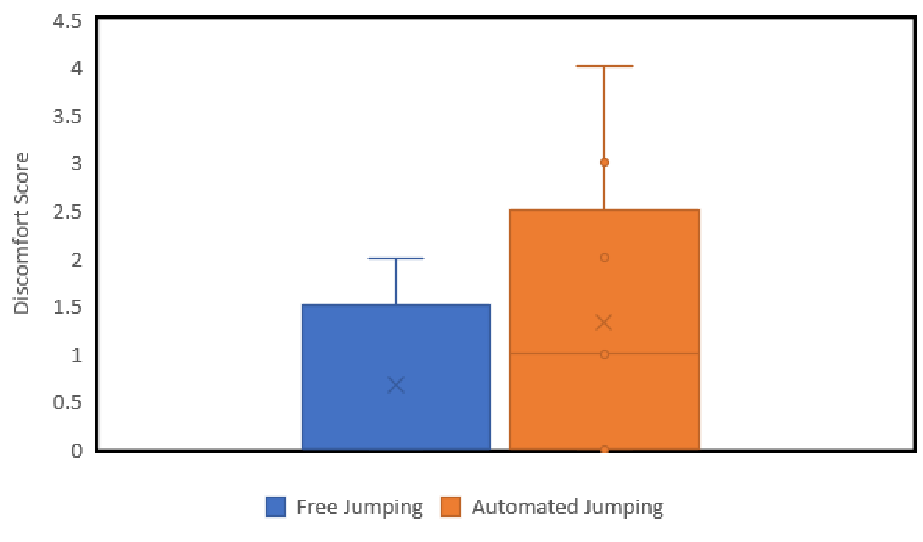
\includegraphics[width=0.46\textwidth]{images/simulator-sickness.pdf}
	(\centering 2)
	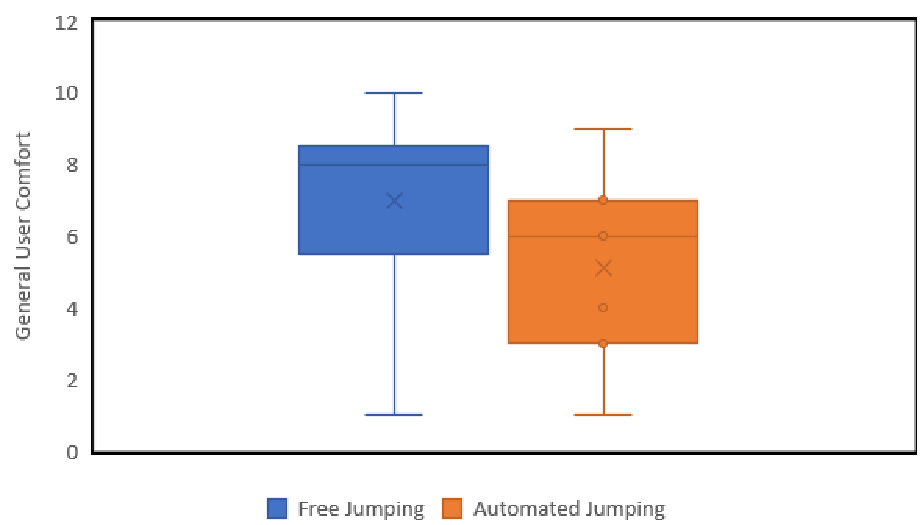
\includegraphics[width=0.46\textwidth]{images/user-comfort.pdf}
	\caption{Box plots illustrating the (1) simulator sickness and (2) user comfort scores reported by participants during each of the study tasks.}
	\label{fig:user-comfort}
\end{figure}

\section{Task Load}
\label{subsection EUS: Task Load}
\acrshort{rtlx} scores were obtained by averaging values from the \acrshort{rtlx} questionnaire for each participant. The scores for both conditions were found to be slightly positively skewed with higher \acrshort{rtlx} scores in AJ ($Avg_{FJ}$ = 26.57, $Mdn_{FJ}$ = 25, $\sigma_{FJ}$ = 17.03; $Avg_{AJ}$ = 36.94, $Mdn_{AJ}$ = 36.67, $\sigma_{AJ}$ = 17.52) as shown in \cref{fig:task-load}. While this disproved \cref{hyp:hyp3} because task load was less for FJ, only 2 out of 9 participants had scores higher than 40 for AJ. This meant that most of these participants still felt that they had less task load even in AJ. There were also 2 out of 9 participants that had lower scores for AJ than FJ.  
\begin{figure}[]
	\centering
	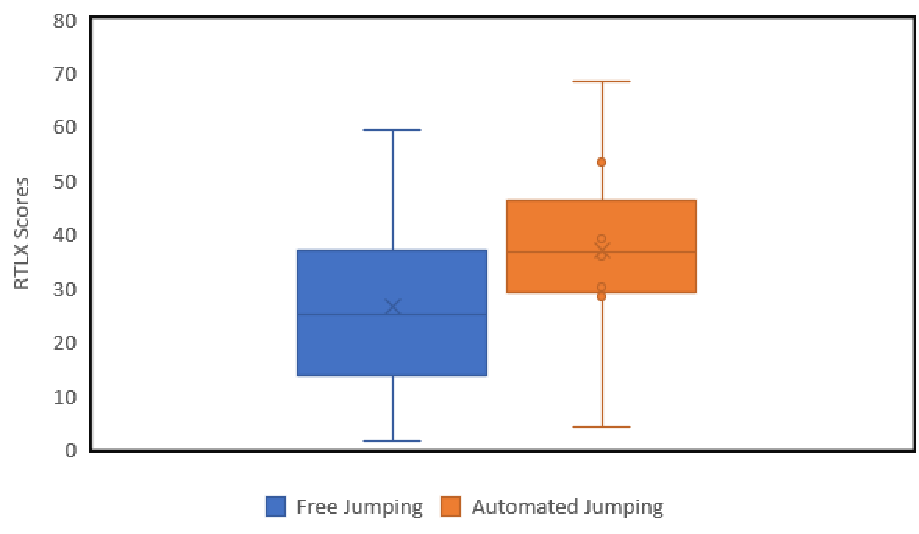
\includegraphics[width=0.8\textwidth]{images/task-load.pdf}
	\caption{Box plot illustrating the \acrshort{rtlx} scores reported by participants during each of the study tasks.}
	\label{fig:task-load}
\end{figure}
\section{Comprehensibility of Jumps}
\label{subsection EUS: Comprehensibility of Jumps}
\cref{fig:jump-comprehensibility} shows that the participants had higher confusion about their position ($Avg_{FJ}$ = 0.89, $Mdn_{FJ}$ = 0, $\sigma_{FJ}$ = 1.17; $Avg_{AJ}$ = 2.89, $Mdn_{AJ}$ = 2, $\sigma_{AJ}$ = 2.52) and orientation ($Avg_{FJ}$ = 2.22, $Mdn_{FJ}$ = 2, $\sigma_{FJ}$ = 2.59; $Avg_{AJ}$ = 5.22, $Mdn_{AJ}$ = 6, $\sigma_{AJ}$ = 2.91) in the AJ condition. Results were positively skewed for position and negatively for orientation in both conditions with FJ having more positively skewed results for position than AJ. 
Despite this proving \cref{hyp:hyp2} wrong we do see that in general the jumps are still comprehensible for AJ and the qualitative answers also show that 8 out of 9 participants did correctly understand how they were getting to the next position and what it would be in the AJ condition. However, only 6 out of 9 participants correctly understood what their next orientation would be when using AJ. Alternatively, all participants correctly understood how to get to the next position, what it would be and what their next orientation would be as well. Nonetheless, it is unclear whether this could have been influenced by the fact that participants may have used \acrshort{hmd}s before in environments where they could freely navigate using controllers and were, therefore, just more comfortable with the technique beforehand. This means that \cref{hyp:hyp2} should be studied again in a different study.

\begin{figure}[]
	(\centering 1)
	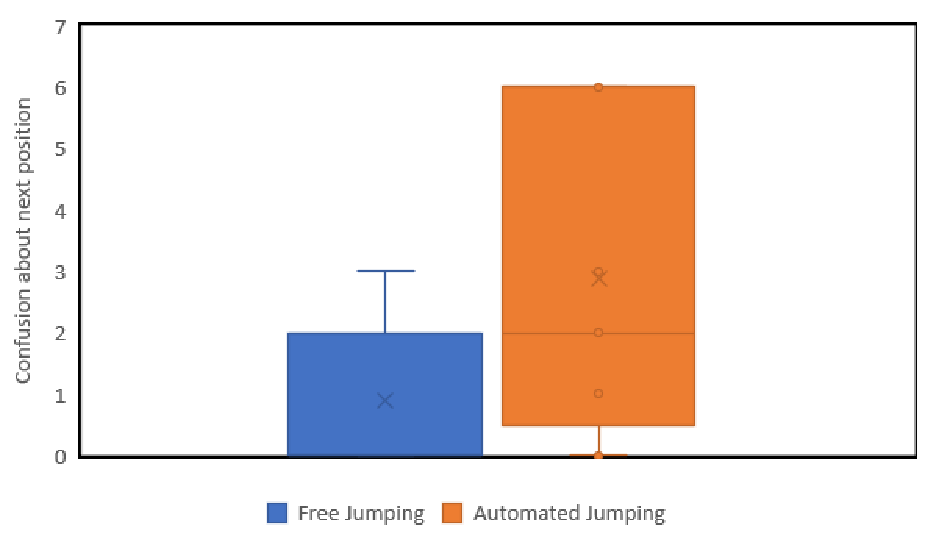
\includegraphics[width=0.46\textwidth]{images/position.pdf}
	(\centering 2)
	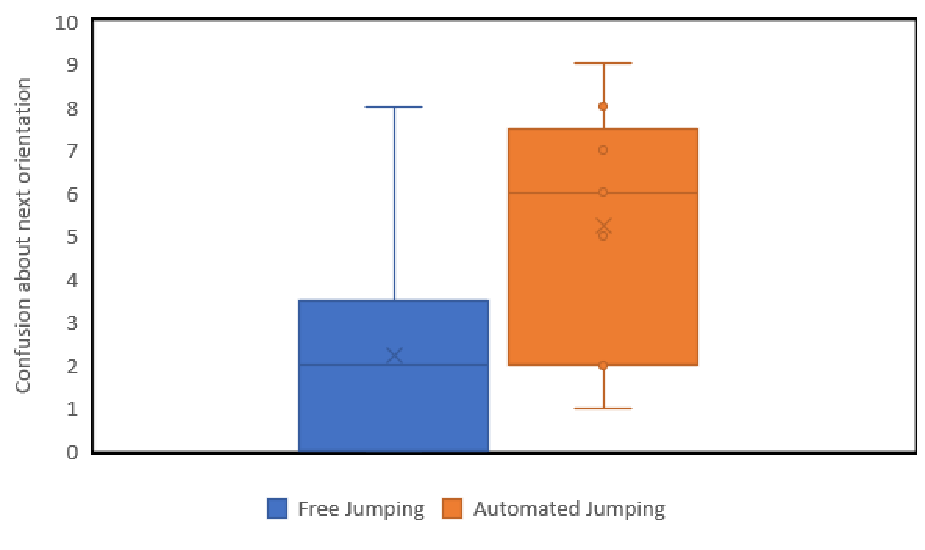
\includegraphics[width=0.46\textwidth]{images/orientation.pdf}
	\caption{Box plots illustrating how often participants felt confused about their (1) next position and (2) next orientation as reported by them during each of the study tasks.}
	\label{fig:jump-comprehensibility}
\end{figure}

\section{Path Recall}
\label{subsection EUS: Path Recall}
The \acrfull{prs}s for both the conditions were very similar
($Avg_{FJ}$ = 37.91, $Mdn_{FJ}$ = 39.01, $\sigma_{FJ}$ = 19.01; $Avg_{AJ}$ = 37.09, $Mdn_{AJ}$ = 39.15, $\sigma_{AJ}$ = 13.69), although it is clear from \cref{fig:path-recall} \acrshort{prs}s have a greater range in the FJ condition with the maximum score being 68.54 compared to a maximum score of 55.63 in the AJ condition. The scores for path recall are also negatively skewed with a more negative skew in AJ. This proves \cref{hyp:hyp4} true.

\begin{figure}[]
	\centering
	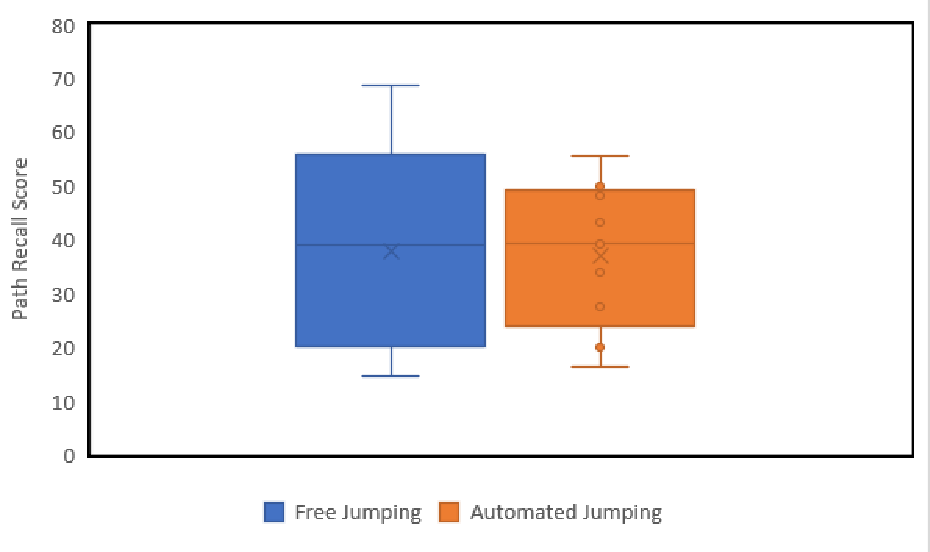
\includegraphics[width=0.8\textwidth]{images/path-recall.pdf}
	\caption{Box plots illustrating the \acrshort{prs} calculated based on the path and objects drawn by participant during each of the study tasks.}
	\label{fig:path-recall}
\end{figure}
\section{Additional Feedback}
\label{subsection EUS: Additional Feedback}
After the questions that were aimed towards answering our hypotheses we also had some further questions on what participants felt about the techniques they were presented with. These qualitative results showed us that 7 out of 9 participants preferred free jumping as shown in the pie chart in \cref{fig:comparison}. However, the reason for this preference was always that the participant had more control when they were using the free jumping technique. As our goal with the automated guided jumping technique is to not allow users to have a lot of control, this preference does not mean that the AJ technique is not relevant. Instead, we can perhaps reconsider the scenario so that users do not feel like they should have control. We also need to think of ways to make users more comfortable with not having as much control. 

Furthermore, even though most participants did not prefer AJ over FJ, 8 out of 9 of them still liked it and had positive things to say about it. For example, $P_8$ preferred FJ and liked it because of \textit{'The feeling of being in control because of moving further and looking around being independent of each other.'}. However, they still liked that AJ gave them the \textit{'feeling of "I can navigate fast without having to do much with the controller and being intuitive with my hand in the air :)'}. Meanwhile $P_5$ liked using their hands when using AJ, $P_9$ found AJ faster than FJ. Both these participants had indicated that their preferred method was FJ due to the control it provided. Participants also understood that there could be scenarios in which AJ would work better. Despite preferring FJ, $P_2$ stated that they would prefer to use AJ in scenarios where the \textit{'virtual public simulations where the hand motions can be kind of universal. Similar to the task example (museums)'}. Therefore, it can be seen that participants just did not prefer it in the scenario of the experiment and wanted more control in this case. This indicated that the scenario was perhaps not an ideal use case for a technique where users should have limited control. There was also some feedback on the AJ technique that can be used to further improve it. This feedback included:
\begin{itemize}
	\item Time between automated jumps should be longer based on feedback from $P_6$.
	\item Gesture tracking was sometimes not precise according to $P_1$.
\end{itemize}

Finally, one realization we had while conducting the study was that participants did not understand that there was a visual countdown for the timer and this may have led to some participants feeling like they were jumping too fast and had limited control. However, this cannot be verified in the scope of this thesis.

\begin{figure}[]
	\centering
	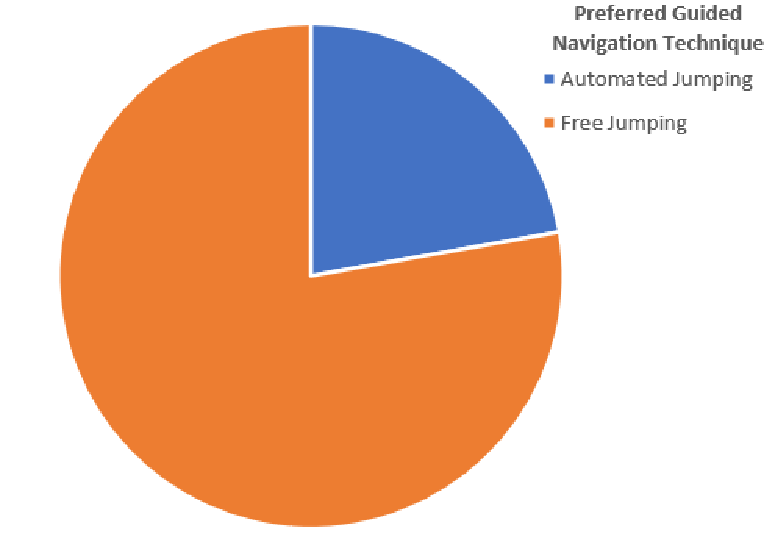
\includegraphics[width=0.6\textwidth]{images/comparison-chart.pdf}
	\caption{A pie chart representing the technique preferred by participants.}
	\label{fig:comparison}
\end{figure}
\section{Further Discussion}
\label{subsection EUS: Further Discussion}
As seen in the previous sections only 1 out of 4 hypotheses were proven true. However, since this was a single study with only 9 participants this does not automatically mean that the automated guided jumping technique does not have its benefits or does not meet the research questions. It is also unclear if the level of experience that participants had with \acrshort{vr} may have effected results. Perhaps in a future study this could be kept consistent either with all participants having barely used \acrshort{hmd}s or those who had quite a bit of experience with using \acrshort{hmd}s. Additionally, the study condition could be changed as well to one that had even less of a focus on navigation and more on the narrative of the environment. This may reduce the need for participants to want more control while navigating as they might want to focus more on the story told by the environment instead of trying to move wherever they want. These are a number of ways in which we can further study our automated guided jumping navigation technique after refining it even more based on the feedback received about it.